% =====================================================================
%  Chapter 3 — The Evidence on Beating the Market
% =====================================================================

\chapter{The Evidence on Beating the Market}
\label{ch:evidence-beating}

Before building anything, it is worth knowing what the best available
evidence says about the thing the machine is supposed to do. This chapter
lays out four findings from the professional and academic literature that
between them define the realistic target for a single investor.

\section{Finding one: most of the published factors replicate}

The most important recent result is also the most encouraging, and it is
encouraging in a way that is easy to misread. Jensen, Kelly and Pedersen,
in the \emph{Journal of Finance} in 2023, reimplemented a large number of
published asset-pricing tests and checked them in samples that had not
been used to form them, across 93 countries.

Their headline is that there is \emph{no general replication\idx{Replication} crisis in
finance}. A majority of published factors replicate in magnitude and sign
out of sample, and the replication rate in the United States was 83.2 per
cent for their sample of characteristics. This is genuinely good news, and
it is the reason a book like this one is worth writing at all.

But the paper contains three further findings that are more useful to this
book than the headline.

The first is that the factors that \emph{fail} to replicate fail for
identifiable methodological reasons rather than at random, and that the
reasons cluster in a small number of characteristics where the original
test was underpowered or where the out-of-sample comparison is intrinsically
hard. The practical consequence is that a factor\idx{Factor}'s replication prospects
can partly be assessed in advance from its construction, and that a factor
built on a clean cross-sectional design with a defensible null is in a
different class from one that is not.

The second is methodological, and it is the one that governs everything in
Parts IV and VI. The researchers compared their own replication results
against what the literature would \emph{predict} if a factor at the margin
were a false positive, and found that the conventional standard errors
were too conservative: factors with marginal statistical significance,
defined in their terms as being two to three standard errors from zero,
reproduced at rates of roughly 0.35 to 0.42 per month rather than the
nearer 0.05 that a five per cent test would imply, with t-statistics in the
range 3.8 to 5.1. In plain terms: a great many published factors are
accepted that should not have been. The same paper makes the companion
point that the capital asset pricing model\idx{Capital asset pricing model}'s expected maximum Sharpe ratio,
given a large number of trials, requires fifteen years of data to invest
at a Sharpe of 0.5, and nearly thirty years at a Sharpe of 2.78. A strategy
that claims a Sharpe of 0.5 has not merely failed to beat the market; it has
also not demonstrated that it is investable.

The third finding is the one that makes the whole enterprise delicate: the
returns of the factors that \emph{do} replicate have weakened over the past
decade. Whatever the cause --- crowding, arbitrage capacity, or a change in
the composition of the investor base --- the direction of the change is
consistent, and it means that a backtest calibrated on the last twenty
years is not a reliable guide to the next twenty.

\begin{figure}[!htbp]
\centering
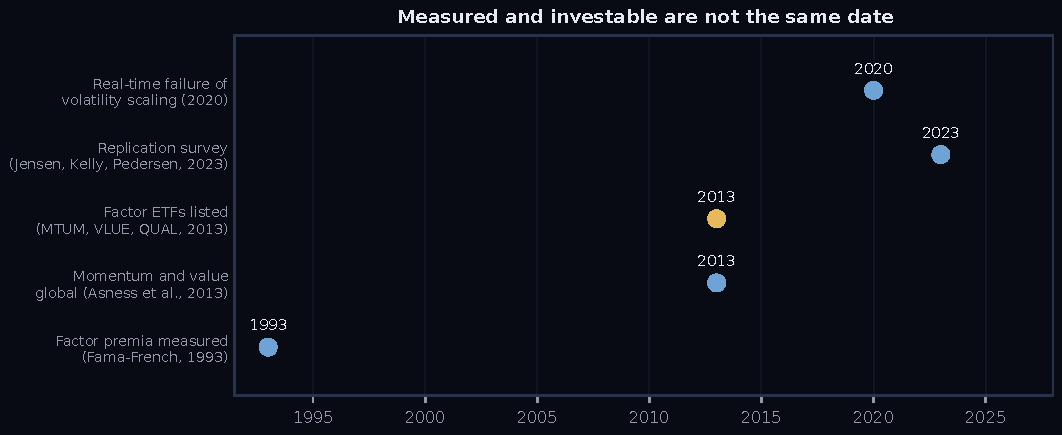
\includegraphics[width=\textwidth]{../figures/fig_premia_timeline.pdf}
\caption{The chronology of the factor literature, with the four findings of
this chapter placed on it: the replication evidence of 2023, the
post-publication decay documented in 2016, the predictor review of 2022, and
the professional underperformance record through 2025.}
\label{fig:premia-timeline}
\end{figure}

\section{Finding two: returns decay after publication}\idx{Decay}

McLean and Pontiff's 2016 study in the \emph{Journal of Finance} is the
single most important data point for anyone planning to act on a published
factor. They took 97 variables with published predictive power, formed
portfolios from them, and then asked what happens to the returns of those
portfolios under two comparisons: before the publication date versus after
it, and in the original sample versus out of sample.

The results were: returns 26 per cent lower out of sample than in sample;
58 per cent lower after publication than before; and 32 per cent of the
decline attributable to the costs of trading, including the market impact of
trading a signal that other people now know about.

The third figure is the one that does not apply to a single investor with
modest size, and it is worth saying why. The 32 per cent is an institutional
number: it includes price impact from large portfolios, and possibly the
effect of a crowded trade in a signal whose participants are institutions
with capacity constraints. A single investor in a liquid ETF has none of
those costs. That is a genuine and quantifiable advantage of the position
this book describes, and it is the mirror image of the advantage the
institutional trader has: the institutional trader can afford to wait for
capacity, while the single investor must accept the decay.

What the single investor cannot escape is the other two thirds: the part of
the decay that is not about trading costs but about the signal itself
weakening once it is known. That is a property of the economics, not of the
crowding, and it is not fixable by being small.

\section{Finding three: a third of the predictors have already died}

Goyal, Welch and Zafirov's 2022 review, published in the \emph{Review of
Financial Studies} in 2024, did the unglamorous work of taking the
predictors of the equity premium in the literature and re-estimating them
in a single consolidated sample. More than one third of them were no longer
statistically significant \emph{in the original sample}. That is, they had
not decayed out of sample; they had stopped working in the sample in which
they had been discovered, which is a stronger condemnation than McLean and
Pontiff's because it removes any ambiguity about out-of-sample design.

The implication for a system builder is precise. If you take a predictor
from the literature, there is a better-than-even chance it is already
dead, and no way to know from the literature itself which one. The
response is to build the predictor yourself from raw prices, over a window
you choose, and to be prepared for the answer to be that it does not work.
That is what Parts III and IV do, and it is why the universe is
deliberately narrow and the features are deliberately elementary: the fewer
things imported from the literature, the fewer ways the backtest can be a
restatement of somebody else's discovery.

\section{Finding four: the profession does not do it either}

The last finding is not academic and it is not about a few dozen factors. It
is about the entire professional industry, and it is the reason a single
investor should not expect that a diligent, well-resourced process will
reliably find an edge.

SPIVA --- the S\&P Dow Jones Indices Active versus Index annual survey ---
is the profession's own scorecard on active management\idx{Active management}, and it measures what
share of active large-capitalisation funds failed to beat
their benchmark over one-, three-, five-, ten-, fifteen- and twenty-year
windows, net of fees, and does so for both the arithmetic and the
risk-adjusted comparison.

Through the year-end 2025 report, 79 per cent of active large-cap funds
underperformed the S\&P 500 in 2025, following 65 per cent in 2024. Over
longer horizons the numbers are more lopsided still: 88.96 per cent
underperformed over five years, 85.59 per cent over ten, 89.93 per cent over
fifteen and 92.89 per cent over twenty. On the risk-adjusted measure the
figures are worse: 95.73 per cent over five years and 98.61 per cent over
ten.

\begin{takeaway}[The base rate]
Across every window the survey measures, the large majority of professional
managers, operating with far more data, more people and more capital than a
single investor, fail to beat a broad index after fees. The prior
probability that a machine-learning pipeline run by one person discovers a
durable, sizeable, net-of-cost edge is not high. The book is written on the
assumption that it is low.
\end{takeaway}

\section{What the four findings jointly imply}

Taken together, these four findings license a specific and unglamorous
strategy, and they are the strategy this book executes.

The replication evidence says that \emph{some} edge exists in published
factors, so the search is not hopeless. The decay evidence says that any
edge found in the literature is probably already gone, so the search must
be conducted on freshly built signals over fresh data. The predictor-review
evidence says that a signal must be re-verified in-sample before it is
trusted out of sample, so the system must be able to do that without
human intervention. The SPIVA record says that the edge, if it exists, is
unlikely to be found by machinery, so the system's expected value cannot
rest on the edge existing.

The last implication is the one that shapes the architecture. If the machine
layer might find nothing, then a system whose core is the machine layer is
a system that might be nothing. The architecture in Part V is therefore
built the other way round: the strategic allocation is a \emph{stated policy},
chosen by argument and held fixed; the machine is permitted to tilt inside
that allocation and nowhere else; and the tilt is sized by the posterior
uncertainty\idx{Posterior uncertainty} of the edge, so that when the evidence is thin the machine
contributes almost nothing and the portfolio is the policy. That is a
system that cannot be destroyed by the failure of its most speculative
component.

\begin{keytakeaways}
\item A majority of published factors do replicate, but the factors that
fail fail for reasons that are knowable in advance, and the standard errors
used to accept new factors are too small.
\item Returns fall by 26 per cent out of sample and 58 per cent after
publication; about a third of that is trading cost, which a small
investor avoids, and two thirds is the signal itself weakening, which no
investor avoids.
\item More than a third of published equity-premium predictors no longer
work even in their own original sample.
\item Most professional managers lose to the index on every long window
measured, net of fees; the prior probability of a single investor finding a
durable edge is low, and the system must be built to survive that.
\end{keytakeaways}
